\documentclass[11pt,journal,compsoc]{IEEEtran}

\providecommand{\PSforPDF}[1]{#1}

\newcommand\MYhyperrefoptions{bookmarks=true,bookmarksnumbered=true,
pdfpagemode={UseOutlines},plainpages=false,pdfpagelabels=true,
colorlinks=true,linkcolor={black},citecolor={black},pagecolor={black},
urlcolor={black},
pdftitle={Making Cheetah Faster},%<!CHANGE!
pdfsubject={Typesetting},%<!CHANGE!
pdfauthor={Alan, Gary, and Dustin},%<!CHANGE!
pdfkeywords={Data Analytics, In-memory database, Concurrency}
}
\usepackage{caption}
% correct bad hyphenation here
\hyphenation{op-tical net-works semi-conduc-tor}
%\usepackage[hidelinks]{hyperref}
\usepackage{hyperref}
\usepackage{graphicx}
\usepackage{subfigure}
\usepackage{textcomp}


\begin{document}
%
% paper title
% can use linebreaks \\ within to get better formatting as desired
\title{Making Cheetah Faster}

\author{Alan~Ng,
        Gary~Chaw,
        Dustin~Kut~Moy~Cheung\vspace{5 mm}\\Department~of~Electrical~and~Computer~
    Engineering\\University~of~Toronto\\\{alan.ng,~gary.chaw,~dustin.kutmoycheung\}@mail.utoronto.ca}
\IEEEcompsoctitleabstractindextext{%
\begin{abstract}
%\boldmath
In this report, we describe how we modified Cheetah, an in-memory database, to speed up queries and insertions using threads. The queries and inserts are transformed into tasks in  a queue and the threads in a threadpool ‘pull’ tasks to execute. Our results show a speedup in query time as the number of threads increase when using the column store. However inserts suffer from the global lock imposed on the store which results in poor performance. Our results show that it is possible to improve the performance of Cheetah by adding more threads and exploiting the different cores in a multi-core processor.
\end{abstract}
}

% make the title area
\maketitle

\IEEEdisplaynotcompsoctitleabstractindextext

\IEEEpeerreviewmaketitle

\section{Introduction}
\IEEEPARstart{T}he need for in-memory databases has exploded in recent years with the
requirement for faster data access to provide near real-time data to users. These types of databases are challenging the dominance of traditional relational databases in an era where multi-core processors and main memory are becoming cheaper.


Unlike traditional databases, in-memory databases do not require optimization of hardware for disk storage, or tweaks to the underlying operating system, allowing an extremely high throughput rate for writes and access using default configurations. In-memory databases do not suffer from unpredictable performance experienced by traditional databases as the seek time required to read data from a hard-drive is eliminated.


Typically in-memory databases are employed when huge amounts of data need to be queried and processed in real-time. An example is a real-time feed of tweets having a specific hashtag for users of the Twitter platform~\cite{twitter}, which requires scanning through millions of tweets posted on Twitter.


Together with the explosion of in-memory databases is the emergence of the JSON data format. JSON has replaced XML as the format of choice for serializing data to be sent in between servers because of native JSON parsing abilities in the Javascript language~\cite{json}. Unlike relational databases, some NoSQL databases allows JSON as input into their system. Examples include MongoDB, CouchDB and Elastic Search. The exploration of mapping JSON data into memory and running queries in parallel still remains an interesting new topic to research to find out if we can optimize the architecture to achieve higher throughput.


\section{Background}
Cheetah inserts data into its store by reading JSON data saved in a file. The JSON data consists of arrays of objects, where each object consists of many name/value pairs. Each of these names might contain values of type: boolean, arrays, number, strings, and other objects. The names in each object are often different from each other, making them unsuitable to be stored in a relational database because of the sparseness of the data.


In a relational database, data is organized into tables, where each table consists of columns. Each column has a particular data type associated with it. The global configuration of tables and the column types is known as the schema of the database.


If one would like to store all of the objects in the JSON data in a traditional database, one of the strategies would be to save the objects into one table, where each column represents all the potential names that the objects can have, and each row represents the object itself. However, this causes huge gaps in our table since most of the time only a few names are present in an object, causing inefficient use of vital memory space.


The Cheetah design explores alternate mappings of JSON data into main memory while making use of relational database paradigms to save data. We describe below the three mappings used in Cheetah to insert the JSON data into the database.


\begin{figure*}
\captionsetup{justification=centering}
\centerline{\subfigure[Column Store]{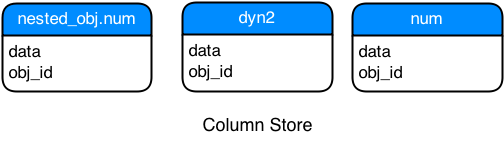
\includegraphics[width=2.5in]{images/column_store} 
\label{fig:col_store}}
\hfill
\subfigure[Row Store]{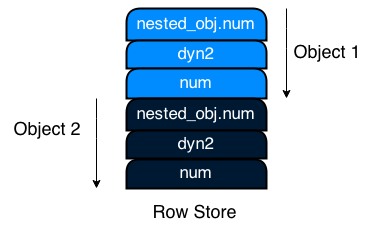
\includegraphics[width=2.5in]{images/row_store}
\label{fig:row_store}}
\hfill
\subfigure[RowCol Store]{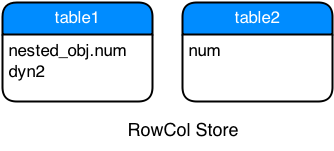
\includegraphics[width=2.5in]{images/row_col_store}
\label{fig:row_col_store}}}
\caption{Different stores layout}
\label{fig:stores}
\end{figure*} 


\subsection{Column Store}
\label{sub:col_store}
The column store (shown in Figure~\ref{fig:col_store}) creates a new table for each name in the object if the table has not been created yet. The table name is the JSON key whose value needs to be saved. To know which value is linked to which object, every object being saved is assigned a unique object id, and each value is then mapped to an object id. As such, the table has two columns, one for the object id and one for the value. This means that the data of an object is broken down and saved in different tables, with the object id as the only connection back to the object.

Those columns are implemented internally by using primitive arrays. The main disadvantage of primitive arrays is that we have to determine beforehand how big the arrays should be, which is not very practical in real-world applications. Other data structures are explored later in this report.

The column store performs better memory-wise compared to the other stores if the objects being stored have sparse names/keys. However, searching data requires more time because we have to scan through all the tables in the store to see if each table has a value for a particular object id.

It would also be interesting to study the impact on cache locality of spreading the JSON data into different tables. In theory, this scheme would affect the cache locality because of the fragmentation of data for a particular object in different memory locations. However, we cannot explore deeper on cache locality due to the lack of appropriate tools to measure cache hit/miss in the JVM platform.

\subsection{Row Store}
As opposed to the column store’s strategy of using multiple tables, only one table is used in the row store (shown in Figure~\ref{fig:row_store}). Each row in the table is mapped to a schema which indicates which row points to which ‘name’ in the object. For example, if there are five names listed in the schema, the first object will store its values in row 1 to row 5, and the second object will store its values in row 6 to row 10 etc.

This scheme is great for searching, since we just need to scan a table to find a particular object with all its name/value pairs. In theory, this greatly improves cache locality. However, this is not very memory efficient since the JSON objects that we save are typically sparse, which means that a lot of rows in our table will be empty, due to a lack of a value for a particular name.

\subsection{RowCol Store}

The RowCol store (shown in Figure~\ref{fig:row_col_store}) is a hybrid store that combines both the row and column store philosophies. It consists of tables, where each table manages a subset of names indicated by the schema for that particular table. This design shares the pros and cons of both the row and column store. It tries to reduce the sparseness of data, while keeping the data not as fragmented into different tables as in the column store. However, there is a need to know which JSON names will potentially be stored beforehand due to the schema requirement for each table.


\subsection{Current Flow of Simple Query Executor}

The main program is the Simple Query Executor and it uses Cheetah\textquotesingle s store engine to store sparse data and run queries on it. The program reads in the JSON data and stores the data depending on the chosen store type: row store, column store, or row-column hybrid store. Then a batch of SQL read-queries is executed. Each query is read and performed sequentially. For each query, the Simple Query Executor program parses the query, then calls the store engine to execute the query. When the store engine executes the query, it overwrites a ResultSet object. The program then prints the results and brief runtime statistics based on what is stored in the ResultSet. This process is repeated for all subsequent queries, which clear and overwrite the ResultSet. Figure~\ref{fig_sequential_query} below illustrates the program flow:

\begin{figure}[!t]
\centering
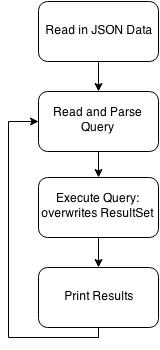
\includegraphics[height=3in]{images/query_sequential}
\caption{Flow of sequential Simple Query Executor}
\label{fig_sequential_query}
\end{figure}

\subsection{Threads}
A thread is the smallest executing context provided by an operating system. At its lowest level, a thread maintains an independent set of values for the processor registers, such as the program counter. This means that threads executing in the same process can potentially share resources such as memory, and instruction code, while executing different parts of the code due to each thread having their own program counter. A single threaded processor switches between different threads by time-division multiplexing to give the illusion of threads running at the same time for the user. More recently with the popularity of multiprocessors, each thread can truly run at the same time by being executed by different processors at the same time.


To run a thread in Java, we can either declare a class that extends the Thread class, or have the class implement the Runnable interface. The advantage of using the Runnable interface is that a class can implement multiple interfaces, but can only extend one class. As such, using the Runnable interface has the advantage of requiring less modifications in their existing class. Another advantage of the Runnable interface is that it can be used directly with Java\textquotesingle s implementation of a Thread pool. 

\subsection{Queries}

Cheetah supports SQL statements for querying data. The querying engine allows users to select some keys/names out of objects, and optionally provide  restrictions where a particular key/name must be of a certain value or range of values while searching for objects. The engine can also return a count of objects that match a certain restriction, Some query types are not supported in Cheetah, like the ‘NOT’ operator, and ‘JOINS’ where different objects can be combined together if one or more of their names/keys match. Currently the ‘UPDATE’ statement is also not supported.


When queries are done without ‘INSERT’ or ‘UPDATE’ statements in between, the use of threads while querying could potentially offer huge speedups since no locks are needed while reading from the arrays. However, an ‘INSERT’ statement will impose a lock on the underlying data structures to avoid any race conditions, and provide the most up-to-date data for the next query. This could potentially affect the performance of threads in that situation.


\section{Analysis of the Store Structure}
As mentioned before in section~\ref{sub:col_store}, a table will contain two columns, one for the object id and one for the value, both implemented using primitive arrays.

There is an intrinsic connection between the object id and the value, where the object id is the ‘key’ to the value. As such, it is natural to explore other data structures that implement a key-value structure, like a Map or a Hash.

We therefore explore the use of Java\textquotesingle s HashMap and TreeMap (which is implemented as a red-black tree, which is always balanced) as alternatives to the array structure. While performing some benchmark tests on these alternate data structures, we notice a significant performance drop.

\begin{figure*}
\captionsetup{justification=centering}
\centerline{\subfigure[Time taken for insersions]{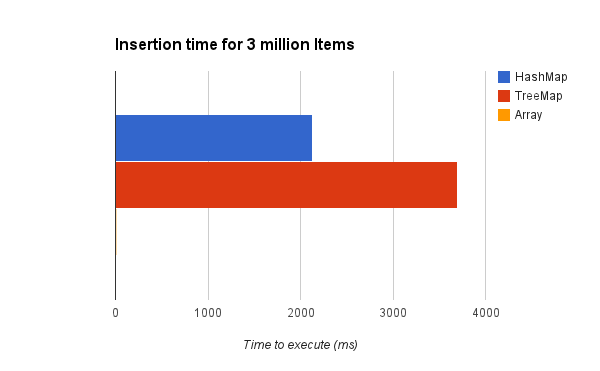
\includegraphics[width=4in]{images/insertion_data_structures.png} 
\label{fig:inserts_data}}
\hfill
\subfigure[Time taken for reads]{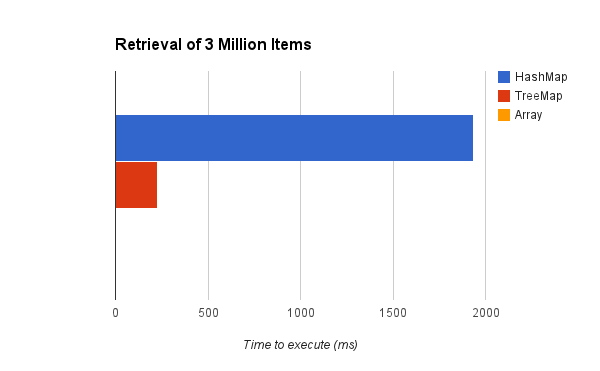
\includegraphics[width=4in]{images/query_data_structures.png}
\label{fig:reads_data}}}
\caption{Time taken for inserts and reads for different data structures}
\label{fig:data_structure}
\end{figure*} 

We can see from Figure~\ref{fig:data_structure} that both the HashMap and the TreeMap take a significant amount of time to insert and read data. The HashMap insertion and reading are expensive since a hash value has to be computed every time.

As for the TreeMap, the insertion is significantly more expensive than reading because each insertion requires a new Tree node object to be created, which is expensive.

Even though, in theory, using a Map or a Hash has architectural desirables, in practice, the overhead required to maintain these structures is very expensive compared to using a simple primitive array. As such, we decided to keep using arrays in our stores for performance reasons, even though the array structure has the disadvantage of being fixed in size.



\section{Implementation}

For the remainder of this report, we will only focus on working with the column store and the new parallelized version of the column store. We focused on the column store because it is excellent memory-wise, while being flexible enough to not require any schema to manage the table layout. 


\subsection{Parallelization of Read Queries}
There are several modifications to the Simple Query Executor and to the store engine in order to support parallel queries. The changes only pertain to query execution. A thread-based approach is chosen to parallelize read-queries. We use the Thread pool implementation provided by the Java standard libraries to re-use existing threads to parallelize queries. Each query is transformed into a task that is then pulled by a free thread in the thread pool. The program modifications have to handle several issues in parallelizing Cheetah and two different program flows were considered to tackle parallelization of read queries. Of the two variants, only one is evaluated.

\subsubsection{Issues with Parallelization}
In the sequential program, each query is performed one after the other. The ResultSet object is cleared and rewritten with each query. For parallel read queries, this ResultSet will need to be multiplied by the number of threads in the threadpool. These result sets were also very large in size. They contained 3 arrays (long, int, and String arrays) and each array pre-allocated space for 100M elements. Given these large arrays, it is very easy to run out of memory on the machines with limited RAM. More swap could be allocated but this would defeat the purpose of developing a program for in-memory databases since swap would introduce reading and writing to the hard-drive and dramatically increase latency.

\subsubsection{Parallel Program Flow}
In the parallel program flow, the Simple Query Executor still starts by reading in the JSON sparse database. Using the thread-based approach, the idea is to have each Query object executed as a runnable object. The program initializes a fixed thread pool that will handle query execution. From this point, two variants of the program were explored to parallelize the Query execution.


In the first variant (shown in Figure~\ref{fig:parallel_print_queue}), an additional thread is created. This thread holds the print queue which accepts queries that have finished execution and will print out results based on the result set’s contents. The query execution itself handles parsing of the query string and execution of the query. This method was deemed not feasible since it requires copying and storing the result set into the query and passing it to the print queue. At the speed the queries were executing, the program easily ran out of memory.

\begin{figure*}
\captionsetup{justification=centering}
\centerline{\subfigure[Parallelized Query Execution with Print Queue]{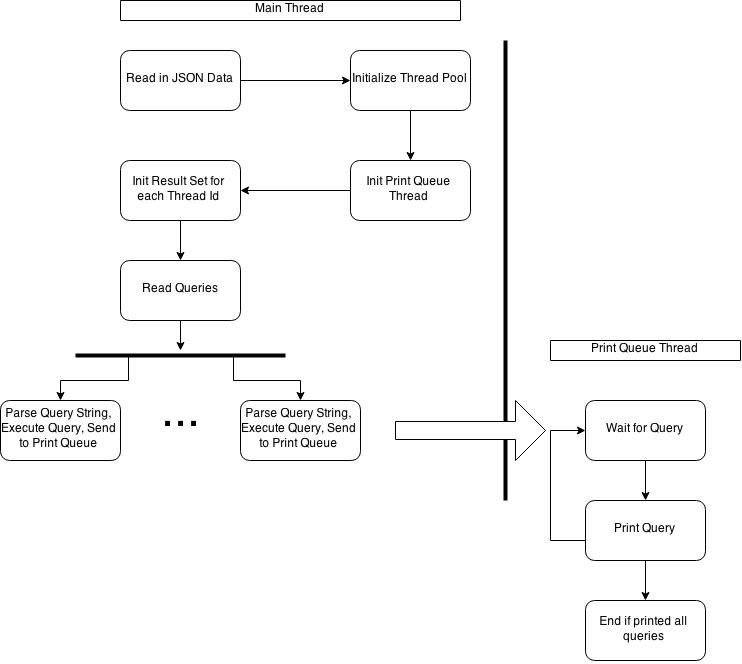
\includegraphics[width=5in]{images/parallel_print_queue} 
\label{fig:parallel_print_queue}}
\hfill
\subfigure[Parallel query execution with result string computation for smaller memory footprint]{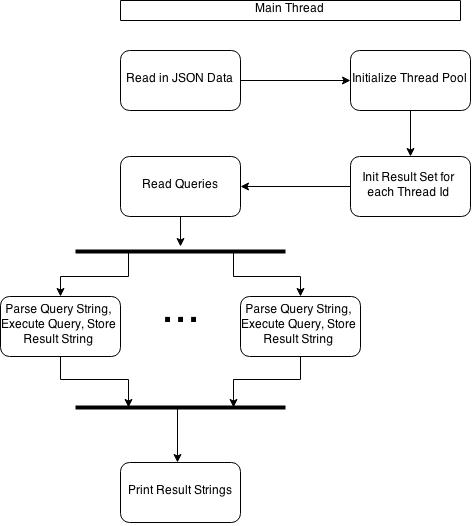
\includegraphics[width=3in]{images/parallel_actual}
\label{fig:parallel_actual}}}
\caption{Parallel architectures chosen for queries}
\label{fig:parallel_query}
\end{figure*} 

In the second variant (shown in Figure~\ref{fig:parallel_actual}), for each thread in the threadpool, an associated ResultSet object is initialized in the store engine. The store engine is modified to contain a map of thread id and result set associations. This initialization was chosen to avoid having each query instantiate their own result sets. Since result sets each contain 3 large arrays, doing so would have been costly. There is no print queue thread in this program flow. Instead, the query handles parsing of the query string, execution of the query, and computing the string that needs to be printed based on the result set. By adding this string computation, we decrease the memory requirements for the query from a large result set to a small string. We also increase the time it takes to finish a query. However, this time was also additional in the original sequential program. Once all the queries have terminated execution, the results from each query are printed one after the other.

The second method above is chosen for our experiments.

\subsection{Parallelization of Writes}
\subsubsection{Enabling Inserts}


The Cheetah implementation provided to us did not support any write operations, only select read queries. In order to explore and experiment in-memory database with read/write mixed workloads as well as concurrency, we have decided to add support for the ‘INSERT’ SQL statement, a write operation.
 
The insert statement adds a new record into the data store from a JSON object, which may be a tree-structure object, compared to traditional SQL-like insert, which specifies the new record in a flattened structure of key-value pairs.

Example JSON object insert statement:

\begin{verbatim}
INSERT {"sparse_942": "haha",
        "nested_obj": {"num": 12, 
                       "pew": "pao"}
       }
\end{verbatim}

Similar to read queries, we have enhanced Cheetah to support parallel execution of insertions.



\subsubsection{Locking}
Concurrency problems such as lost update, uncommitted dependency and inconsistent analysis can be solved by implementation of locking~\cite{krueger2010data}\cite{garcia1992main}. We have explored and implemented both of the following two locking models:
 
Simple lock: A mutex lock is placed to protect the data so that a write transaction needs to acquire lock on the data before it writes the data. Therefore, any addition and modification of elements into the data store must be inside a lock-protected critical region to prevent concurrent writes to the same data. However, read transaction is not required to acquire the lock on the data.
 
Reader-writer lock: readers block writers but permit other readers, and writer blocks readers and writers. A read transaction will acquire a shared lock on the data before it starts reading data. And a write transaction will acquire an exclusive lock before it starts writing data.
 
Different from the update statement which modifies one or more existing entries in the data store, the insertion statement simply appends new entries to Cheetah data store. Since there is no other write operation other than insertion allowed in the current Cheetah implementation, we aim to protect against the potential conflict concurrent insertions by two or more threads.

\subsubsection{Lock Granularity}
Coarse-grained lock: A single lock at data store (table) level. Any insertion of a new record will result in locking the entire data store. If another insertion needs to add a different record to the data store, it is forced to wait until the first transaction exits the critical region.
 
For a simple lock, a ReentrantLock is created when the data store is initialized. The lock is acquired by the thread before the JSON object is inserted to the data store, inside InsertObject(), or before the scan process begins for a select statement.  The lock is released after the entire JSON object has been inserted, or the results set have been gathered for the select statement.

For Reader-Writer lock, A ReentrantReadWriteLock is created when the data store is initialized. A reader (shared) lock is acquired for read queries and writer lock is obtained for write queries; the locks are released once the operation is completed.
 
Fine-grained lock: One lock per data column in data store. Instead of having just one single lock protecting the entire data store, there will be one lock per data column
 
For simple locking, a ReentrantLock is created when the column object is initialized. The lock is acquired by the thread before the column value of the inserted record is added to the column store, in saveStrValue(), saveBoolValue(), saveDoubleValue(), and saveLongValue().
 
For reader-writer lock,  a ReentrantReadWriteLock is created when the column object is initialized. The reader lock is acquired before the scan process begins on the column data items, and writer lock is acquired before a new data item is added to the column store.



\subsubsection{Support of other types of write transactions}
Due to limited time span of this project, we did not implement functionalities to support other types of write operations such as update, which modify one or more existing records, and delete, removal of existing records in data store.


\section{Experimental Results}
These tests were run on a machine with 32 cores (Intel Xeon CPU E5-2660 at 2.2Ghz) with 47GB of RAM. For each test, the average of 5 runs is recorded.

\subsection{Parallel Read Queries}

\begin{figure*}
\captionsetup{justification=centering}
\centerline{\subfigure{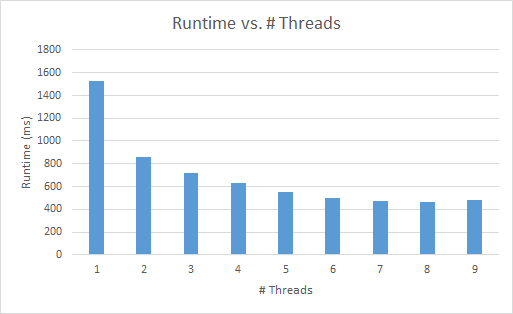
\includegraphics[width=4in]{images/runtime_vs_threads} 
\label{fig:runtime_vs_threads}}
\hfill
\subfigure{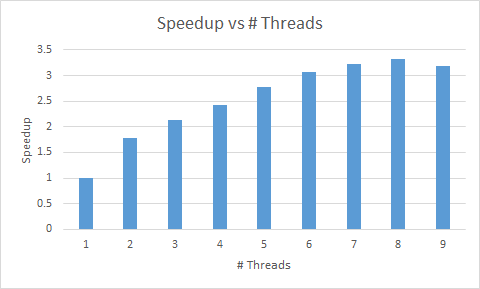
\includegraphics[width=4in]{images/speedup_vs_threads}
\label{fig:speedup_vs_threads}}}
\caption{Runtime and Speedup vs number of threads for parallel program flow}
\label{fig:speedup_reads}
\end{figure*} 

We compared the performance of parallel read-queries to that of sequential queries. In our experiment, we measure the total runtime to read and execute 50 queries in the original sequential program and in the new parallel program. The runtime data is collected for the parallel program running between one thread up to nine threads. In the charts below, the runtime and speedup is shown for the parallel program. As expected, the runtime decreases as we increase the number of threads in the thread pool as shown in Figure~\ref{fig:speedup_reads}. With one thread, the runtime is approximately 1500 ms, whereas with two threads the runtime is approximately 850 ms. We notice, however, that as more threads are added, we get diminishing returns in performance gains. This is more evident in the speedup graph. There is a near 2X speedup between one thread and two threads, and from three threads to eight threads, the speedup still increases but with smaller gains with each thread added. Finally at nine threads, there is actually a slowdown compared to running the program with eight threads. The diminishing gains can be attributed to context switching and cache misses as the number of threads increase. As the number of threads increase there is more contention so the cache gets rewritten more often in order to process the individual queries. We note that in the read-queries case, there should be no lock contention as it is assumed that no other queries are inserting or updating tables in the store engine.


It\textquotesingle s interesting to note that there was also a significant performance increase between the original sequential program and the parallel program running with one thread. The original program executed all 50 read queries in approximately 7000 ms whereas the parallel program running on one thread required only 1500 ms. This discrepancy is perhaps due to the order in which query parsing, execution and result printing is performed. In the parallel program, all printing happens after all queries have been executed. The string to be printed were computed during parallel processing, however the actual print to standard output occurs sequentially in the main thread. In contrast, the sequential program computes the string to print and prints the string immediately after each query is executed. This causes many I/O synchronizations to occur during the batch execution of queries and slows down the program. We used the YourKit Java profiler to get an estimate of the time it takes to execute and print queries. This profiler estimates the amount of time spent in each function in each thread. For the purposes of this experiment, we only took into account functions that were related to cheetah and focused on the execution of queries and the printing of results.

\begin{table*}
  \centering
  \begin{tabular}{ |l || c | c |}
    \hline
     & \% of time for original sequential program & \% of parallel time for parallelized program (with 1 thread) \\ \hline\hline
    Executing Query & 9\% & ~0\% \\ \hline
    Printing Summary & 47\% & 15\% \\
    \hline

  \end{tabular}
\caption{Speedup for query execution and printing}
\label{table:speedup}
\end{table*}


We see from Table~\ref{table:speedup} that a simple reorganization of the program flow achieves significant performance gains. In the sequential program, Query execution and result printing accounted for 9\% and 47\% of the execution time respectively. In the parallel program running with one thread, the query execution time was nearly undetectable by the Java profiler and the printing of results accounted for 15\% of the execution time. 


\subsection{Parallel Inserts}
Results demonstrate the performance gain when threading is used to parallel process 10K insertions. As shown in Figure~\ref{fig:simple_lock}, there is a reduction of 36\% in execution time when two threads are used instead of one. However, as number of threads increase, the performance gain is diminishing. The performance starts to deteriorate gradually when more than seven threads are used.

\begin{figure}[!t]
\centering
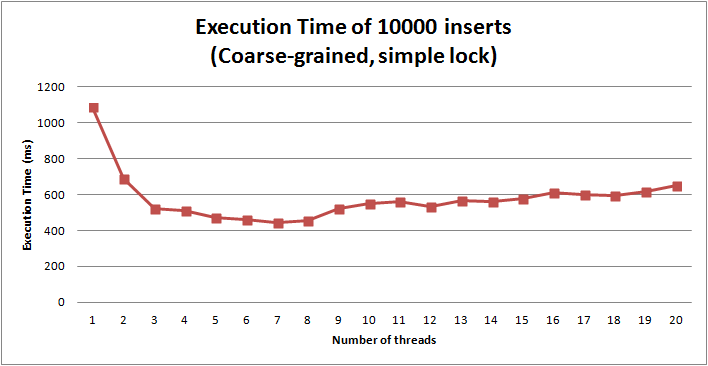
\includegraphics[width=3.5in]{images/simple_lock}
\caption{Time taken to execute 10000 insert statements, into column data store protected by simple locking mechanism (coarse-grained) }
\label{fig:simple_lock}
\end{figure}


At first glance the results look abnormal, as the speedup seems not possible as the coarse-grained lock implemented at the data store level would allow only one thread writing to the database at a time. As a result, parallel execution of inserts should bring no performance improvement. However, we discovered most of the time spent when executing the insert statement is on reading, parsing and flattening the tree-structured JSON object (using recursive functions). Parallelization helps with those tasks.


\subsubsection{Evaluation of Lock Granularity}

Another experiment we conducted is to compare the performance impact of coarse-grained vs. fine-grained lock. Our results show use of fine-grained lock increases execution time. As shown in Figure~\ref{fig:thousand_inserts}, use of fine-grained locks introduces overhead, which is not seen when only a single lock (coarse-grained) is deployed. However, based on our experiment configuration, we do not observe the performance improvement when using fine-grained lock to protect individual data column, vs. coarse-grained lock to protect the entire data store.

 
At this stage, based on available data, one theory to explain the results is the actual time taken to execute the store procedures is too small a fraction. Therefore, the contention rarely occurs regardless of the sparseness (or density) of the data.


\begin{figure}[!t]
\centering
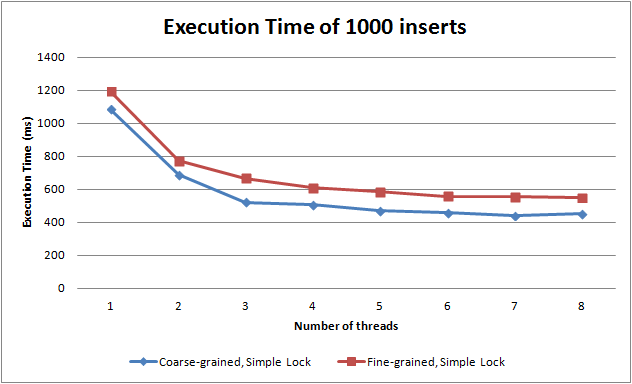
\includegraphics[width=3.5in]{images/execution_thousand_inserts}
\caption{Performance-wise, coarse-grained locking seems to be always better than fine-grained locking}
\label{fig:thousand_inserts}
\end{figure}


\subsubsection{Evaluation of Simple Lock vs Reader-Writer Lock}
We tested the performance of the two locking protocols: single mutex lock and Reader-Writer lock. To do this, we created a workload which consists of 50\% insert statements and 50\% read queries. 

Our results show that reader-writer lock seems to always perform better than simple lock (see Figure~\ref{fig:mixed_load}). This is inline with our expectation, as simple lock blocks all concurrent threads attempting to read and write, while reader-writer lock permits concurrent read operations but only blocks everyone else when one thread acquires the writer/exclusive lock.

\begin{figure}[!t]
\centering
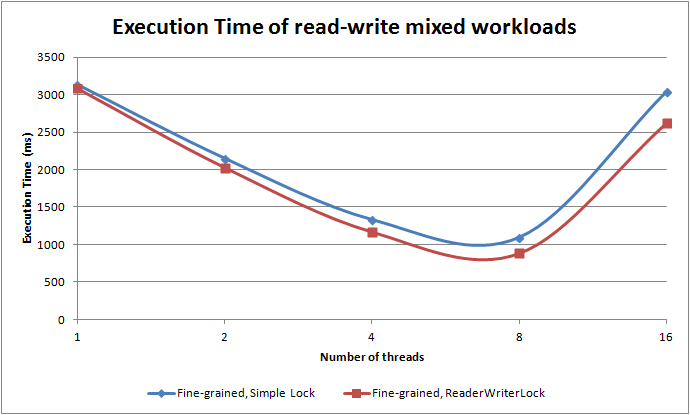
\includegraphics[width=3.5in]{images/mixed_load}
\caption{Reader-Writer locks seems to perform better than simple lock.}
\label{fig:mixed_load}
\end{figure}


\section{Related Work}
Other approaches for in-memory databases have been previously studied. Redis is one of them. Redis is an open-source cache and store that is used extensively in the industry. Even though Cheetah stores JSON data, the JSON format is still very similar to a key-value format, where each attribute in the JSON object is a key. Redis is famously single-threaded and deals with all network query (and write) requests by using non-blocking IO coupled with an event-loop approach, which allows Redis to have a high throughput. There is a possibility to run Redis in a multi-process fashion by using Redis Cluster~\cite{redis-cluster}. This allows the Redis database to be spanned across several machines.

Redis uses an adaptive scheme to save their key-value data. The most natural way of storing this data would be by using a highly-efficient hash structure.. However, for small key-value storage, they instead just encode them in an O(N) data structure, like a linear array with length-prefixed key value pairs~\cite{redis}. The hash will be converted into a real hash table as soon as the number of elements it contains becomes too large. Since a linear array of key value pairs happens to play very well with the CPU cache~\cite{redis} (it has a better cache locality than a hash table).

On the data partitioning side, HYRISE~\cite{hyrise} is another in-memory database system that adopts a hybrid system for storing data. It dynamically partitions tables of varying widths depending on the most accessed columns. This contrasts with Cheetah which requires a schema to determine the layout of its tables for both the row and the rowcol store. HYRISE will alter their partitioning based on the nature of the queries. If there are queries that perform sequential scans (for example, to find values of a column who are within a range), they determined that narrow partitions perform better because of the improved cache locality. For operations that require a lot of inserts, updates or deletes, a wider partitioning is favored. Using a model that is able to predict the performance of the different partitionings, HYRISE will change the partitioning according to the nature of the queries. 


The Argo Document store~\cite{argo} is the closest architecturally to the functionality and store design of Cheetah. They employ a very simple store that deconstructs the attributes in JSON data into keys and use a single table to store the object id, the key and its value. Similar to Cheetah, it also supports querying via SQL statements and supports INSERT, DELETE, JOINS, and SELECTs. Argo also uses threads while querying with JOINs, but doesn’t use threads for querying in general.


\section{Conclusion and Future Work}
Use of threads has significantly improved the time it takes to run queries. We are able to improve the performance while keeping most of the Cheetah architecture relatively unchanged. We also experimented with different lock mechanisms and observed some gains. We also explored the various data structures that we could use in our table before using primitive arrays due to its superior performance for inserts and reads.

Future work needs to be done to experiment with different JSON data mappings to memory to exploit multi-threading while preserving cache locality. Due to lack of existing analysis tools for the JVM platform, this task remains hard to do.  Finally, two of the data stores remain unmodified in our work. Namely the row store and the rowcol store could be modified using the same architectural changes we performed for the column store, to exploit multi-threading and observe how these stores perform in these situations.

The use of different types of queries, and their impact on the multi-threaded design should also be explored in the future. In our current work, we only performed queries on ‘SELECT WHERE’ types. Other query types could provide better insight on the behaviour of threading in the current data stores, and perhaps provide hints on a potential new store configuration that could provide better gains for threaded queries. 


% use section* for acknowledgement
\ifCLASSOPTIONcompsoc
  % The Computer Society usually uses the plural form
  \section*{Acknowledgments}
\else
  % regular IEEE prefers the singular form
  \section*{Acknowledgment}
\fi

First and foremost, we would like to thank Professor Cristiana Amza and our Teaching Assistant Sahel Sharify for their guidance and pointers provided throughout the course of the project. 


We are also grateful to Alan Lu  who orchestrated the original Cheetah design and was kind enough to allow us to contribute to this wonderful project.


Lastly, to the entire class of ECE1747 who made this course an awesome learning experience.

% Can use something like this to put references on a page
% by themselves when using endfloat and the captionsoff option.
\ifCLASSOPTIONcaptionsoff
  \newpage
\fi

% references section
\bibliography{cheetah_report}
\bibliographystyle{ieeetr}

% can use a bibliography generated by BibTeX as a .bbl file
% BibTeX documentation can be easily obtained at:
% http://www.ctan.org/tex-archive/biblio/bibtex/contrib/doc/
% The IEEEtran BibTeX style support page is at:
% http://www.michaelshell.org/tex/ieeetran/bibtex/
%\bibliographystyle{IEEEtran}
% argument is your BibTeX string definitions and bibliography database(s)
%\bibliography{IEEEabrv,../bib/paper}
%
% <OR> manually copy in the resultant .bbl file
% set second argument of \begin to the number of references
% (used to reserve space for the reference number labels box)

% \begin{thebibliography}{1}

% \bibitem{IEEEhowto:kopka}
% H.~Kopka and P.~W. Daly, \emph{A Guide to {\LaTeX}}, 3rd~ed.\hskip 1em plus
  % 0.5em minus 0.4em\relax Harlow, England: Addison-Wesley, 1999.

% \end{thebibliography}

% that's all folks
\end{document}
